\section{Theorie}
\label{sec:Theorie}

\cite{sample}

Ein Laser ist monochromatisches Licht hoher Kohärenz und Intensität. Er besteht grundlegend aus drei
Komponenten, einem aktiven Lasermedium, einer Pumpquelle und einem Resonator.
Das aktive Lasermedium, in diesem Versuch ein Helium-Neon Gemisch, eignet sich zur Erzeugung
von Laserlicht durch stimulierte Emission. Die Pumpquelle sorgt für eine Besetzungsinversion im Gasgemisch.
Der Resonator lässt den Laser in das aktive Lasermedium zurück koppeln, wodurch ein
selbst erregender Oszillator entsteht.

\subsection{Entstehung von Laserlicht}
Eine Pumpquelle führt dem Helium permanent Energie zu, welche es durch Stöße an
die Neonatome abgeben und diese in einen angeregten, metastabilen Zustand versetzen.
Trifft ein Photon auf ein angeregtes Neonatom kann es zur stimulierten Emission kommen, dies
bedeutet, dass das Neonatom, unter Aussendung eines Photons mit gleicher Energie, Phase und
Ausbreitungsrichtung wie das erste, in den Grundzustand zurückkehrt. Durch die Besetzungsinversion soll
die stimulierte Emission häufiger auftreten als die spontane Emission, bei der ein Neonatom aus
dem Grundzustand ein Photon absorbiert und dieses wieder aussendet, wodurch der Laser eine hohe
Kohärenz bekommt.

Der entstehende Laserstrahl wird durch den optischen Resonator, welcher aus zwei Spiegeln besteht,
in das aktive Lasermedium zurückreflektiert. Einer der Spiegel ist halb durchässig, wodurch der
Laser ausgekoppelt wird. In Abbildung 1 ist die Funktionsweise schematisch dargestellt.

\begin{figure}[H]
  \centering
  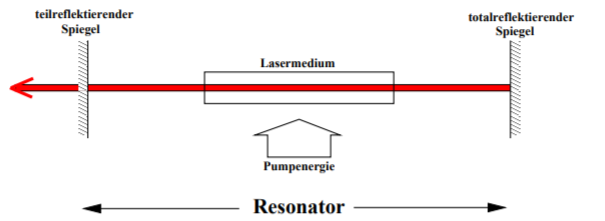
\includegraphics[height=6cm]{Lasermedium.PNG}
  \caption{Schematische Darstellung eines Lasers \cite{sample2}}
  \label{fig:Lock}
\end{figure}


Der Resonator ist genau dann optisch stabil, wenn seine Verluste
kleiner sind als die Verstärkung durch die stimulierte Emission. Es gilt dann:
\begin{align}
  &0 < g_{\symup{1}} \cdot g_{\symup{2}} < 1 \\
  \\
  &\text{mit} \:\:\:\: g_{\symup{i}} = 1 - \frac{L}{r_{\symup{i}} }
\end{align}

Dabei ist $L$ die Resonatorlänge und $r_{\symup{i}}$ ist der Krümmungsradius der Spiegel.
Geringe Verluste im Resonator können durch das Zusammenfallen der Spiegelbrennpunkte erreicht werden.

\subsection{Schwingungsmoden}
In dem Resonator wird die Anzahl $q$ an Wellenlängen des Lasers longitudinale Mode bezeichnet. Durch
Verkippungen und Spiegelunebenheiten kann der Resonator auch in transversalen Moden schwingen.
Seine Eigenschwingungen werden mit TEM$_{\symup{lpq}}$ bezeichnet. Hierbei sind $l$ und $p$
die Knoten in x- und y-Richtung und q die longitudinale Modenzahl. Niedrige Moden
haben eine höhere Symmetrie und weniger Verluste als hohe Moden, weshalb die Grundmode
TEM$_{\symup{00}}$ am besten darstellbar ist. Die Intensitätsverteilung dieser Mode
ist gaußförmig.
